\documentclass[a4paper, twoside, 11pt]{article}
 \usepackage[margin=2.5cm]{geometry}
 \usepackage[]{xcolor}
 \usepackage{cite}
 \usepackage{graphicx}
% define the title
\author{C. ~Han, R. ~Jones, L. ~Towell}
%defines the title
\title{Insert Literature Review Title}
\begin{document}
	%generate the title
	\maketitle
	
	\begin{abstract}
		Here we can write an abstract of between 100 - 150 words about the subject of the article. make all of your changes here 
	\end{abstract}
	%insert the table of contents
	\tableofcontents
	
	\section{Project Brief}
	The project will involve the design and implementation of an artificial intelligence based system for the automated recognition of faces, emotions, or gestures using existing public domain image datasets. The system will employ dimensionality reduction algorythms, such as component analyses or projective transforms to extract useful feature information, and also different machine learning algorithms to automatically classify the generated features to the different classes.
	\section{Introduction}
	Introduction to the paper: what does the paper do, what is the topic that we are discussing have we touched on any notable points or pieces of research that is worth mentioning?
	\section{Related Work into this Litrarture Review}
	I believe that this section will outline the information that we have taken from previous literature reviews around the subject of machine learning and facial recognition / Emotion recognition using AI.
	\section{Outline}
	\ldots{} I have no idea what the difference between an outline and an introduction is.
	\section{Main Body of the Literature Review}
	\ldots{} and here is the main body of our research and our findings from the literature review. \
	
	\subsection{Introduction to machine  learning / what is a neural network.} - Ricky
	\subsection{Evolution of machine learning  and deep neural networks} - Luke
	 machine -> several machines -> Autonomous Machines
	
	
	\subsection{ Evolution of machine learning  to recognise facial features in images, facial features in video, facial  features in real time.} - Ricky
	
	\subsection{ Why are we looking into the  use of machines to identify human emotions?} - HCI - What sort of systems  will it be useful in. - Luke
	\subsection{How can it be used in society? }- Ricky
	\subsection{Ethical / social implications  of emotion recognition and analysis.} - luke
	\subsection{How are these Experiments and  studies conducted.}- Ricky
	Gathering of data
	\subsection{FACS} - 6 Agreed emotions -  Explain what FACS is and why it is so significant. - Luke
	\subsection{Definition of data models  and use of datasets} - Ricky
	\subsection{Training of machines} - Luke
	\subsection{Configuration of machines} - Ricky
	\subsection{Testing of machines} - Luke
	\subsection{Evolution of types of data  being used to identify emotion?} -Ricky
	Facial - Do you want to split these up or do you want to keep them together to make sure that the dialogue flows better?
	Body
	Audio
	Physiological
	\subsection{Typical future work that is  highlighted in studies} - How should we move and advance the recognition of  emotions in society. Feedback to people how others are feeling using  google glass. - Luke
	How to install an image in the file:\\
	\begin{center}
	\centering %This is one of the many ways to center something in Latex
	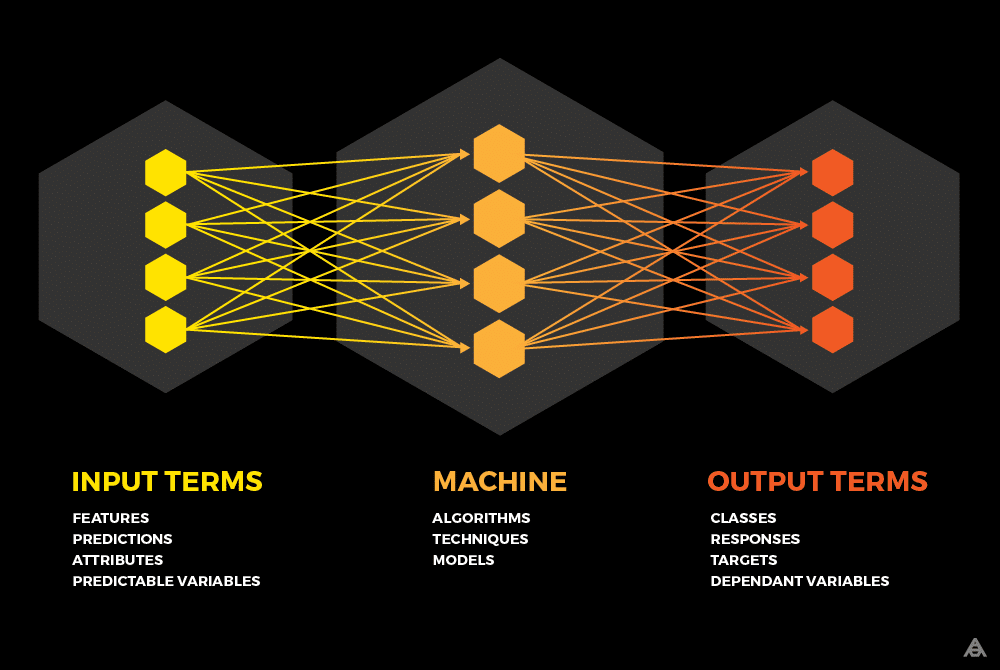
\includegraphics[scale=0.25]{images/understanding-machine-learning} % This is how to insert an image from the images folder that I have created in the repo.
	\end{center}
	\section{Summary of the Literature Review \& Future Work}
	\ldots{} Summary of the Literature Review and the future work that we would be able to look into in order to find more information or the next steps after we have produced the literature reviw. I think this might include progressing to actually attempt to produce some form of convolusion neural network in order to creat our own facial / gesture recognition system.
	
	Here is an example of referencing.
	Blablabla said Nobody ~\cite{Nobody06}.
	
	\bibliographystyle{alpha}
	\bibliography{LiteratureReviewBib.bib}{}
	
\end{document}